\documentclass[11pt,a4paper]{article}

\usepackage[margin=2.5cm]{geometry}
\usepackage{amsmath,amssymb}
\usepackage{booktabs}
\usepackage{graphicx}
\usepackage[T1]{fontenc}
\usepackage[utf8]{inputenc}
\usepackage{microtype}
\usepackage{parskip}
\usepackage[dvipsnames,svgnames,table]{xcolor}
\usepackage{hyperref}
\hypersetup{
  colorlinks=true,
  linkcolor=MidnightBlue,
  citecolor=MidnightBlue,
  urlcolor=MidnightBlue,
  pdftitle={QC gaps: H2 diagnostic and ethylene exploration in inZOR-ND},
  pdfauthor={Dumitru Novic},
  pdfkeywords={quasi-degeneracy, SA-CASSCF, excitation gap, ethylene, hydrogen, inZOR-ND, quantum chemistry}
}
\usepackage[numbers,sort&compress]{natbib}
\usepackage{caption}
\usepackage{enumitem}

%% Brochure figures (dev). For arXiv upload, copy PNGs into ./figures/ and put that path first.
\graphicspath{{../../web/brochure/tests/qc_gaps_h2_ethylene_unified/figures/}{./figures/}}

\title{\textbf{Electronic Gaps Near Quasi-Degeneracy:\\[0.25em]
Minimal \texorpdfstring{H$_2$}{H2} Diagnostic, Ethylene Exploration in \mbox{inZOR-ND},\\[0.15em]
and the Discrete-Search Benchmark Boundary}}

\author{
  Dumitru Novic\\[0.2em]
  \textit{Independent Researcher}\\[0.2em]
  \small\href{mailto:dumitru.novic@gmail.com}{dumitru.novic@gmail.com}
}

\date{April 2026}

\begin{document}
\maketitle

\begin{abstract}
Near \textbf{quasi-degeneracy}, multi-reference methods depend critically on the
\textbf{active space}. Poor orbital choices can distort \textbf{excitation gaps}
and state orderings long before a full potential-energy surface is trusted.
This note unifies two complementary \textbf{inZOR-ND} threads under the same
chemical motif---gaps under electronic stress---while keeping their
\textbf{algorithms and claims} distinct.

First, we document a \textbf{minimal H$_2$ diagnostic}: a seven-point H--H
stretch (cc-pVDZ) with \textbf{SA-CASSCF(2,2)} HOMO--LUMO gaps comparing active
MO indices chosen by \textbf{inZOR-ND} to a \textbf{NOON}-style rule. The inZOR-ND
track yields a \textbf{monotone} gap curve across the scan; the NOON-tracked pair
does \textbf{not}, with a documented spike at $R=2.0$~\AA\ ($\sim$18.14~eV)
versus $\sim$2~eV at neighbouring points.

Second, we summarise \textbf{ethylene} near torsional quasi-degeneracy in the
\textbf{continuous exploration} stack: SA-CASSCF(2,2) gap-style observables feed
an evolving population (2D/3D, multiple seeds, score variants) in the dedicated
scene \texttt{scene\_ethylene\_quasidegen}. We reference exported validation
figures and a separate \textbf{3D regional} technical report on multi-basin
low-gap structure, discovery speed versus uniform control, and reproducibility
limits for identical probe traces.

We state \textbf{claim hygiene}: continuous population logs must not be cited as
\textbf{discrete orbital-set search} benchmark outcomes. Large-scale discrete
comparisons (e.g.\ eight-benchmark suite including ethylene SA-CASSCF and
N$_2$) remain the citation target for CAS discovery claims~\citep{inZORNDActiveSpace2026}.

All tabulated H$_2$ numbers are frozen in machine-readable JSON alongside the
public HTML companion~\citep{inZORNDQCGaps2026}; the 3D ethylene regional study
is published as a sibling page~\citep{inZORNDEthylene3D2026}.
\end{abstract}

\section{Motivation}
Multi-reference models are sensitive to orbital partitioning: the same nominal
method can produce qualitatively wrong gaps along a dissociation coordinate if
the active pair is misidentified~\citep{Helgaker2000Molecular}. Practical
workflows therefore need \textbf{cheap diagnostics} that stress-test gap
behaviour before expensive dynamics or extended surfaces.

\textbf{inZOR-ND} is used in this work in two senses that share a scientific theme
(gaps near quasi-degeneracy) but differ in implementation:
\begin{itemize}[itemsep=2pt]
  \item \textbf{Discrete search} over candidate active spaces (orbital index
        sets), as in published CAS benchmarks~\citep{inZORNDActiveSpace2026}.
  \item \textbf{Continuous exploration}: internal coordinates evolve under
        selection pressure with quantum-chemistry probes scoring each proposal
        (ethylene scene).
\end{itemize}
Confusing the two would mis-state what was validated where; we keep the
boundary explicit throughout.

\section{Methods}

\subsection{H$_2$: seven-point SA-CASSCF(2,2) gap scan}
Hydrogen in a minimal (2e, 2o) active space isolates \textbf{orbital-choice
effects} on a single gap observable without conformational degrees of freedom.
We use PySCF-based SA-CASSCF(2,2)~\citep{Sun2018PySCF} in the cc-pVDZ basis at
bond distances $\{0.7, 0.9, 1.1, 1.3, 1.6, 2.0, 2.5\}$~\AA. Two orbital
choices are compared:
\begin{itemize}[itemsep=2pt]
  \item \textbf{inZOR-ND track:} active MO indices $(0,1)$.
  \item \textbf{NOON-style track:} indices $(0,3)$ for this documented run.
\end{itemize}
HOMO--LUMO gaps (eV) and monotonicity flags are archived in
\texttt{h2\_stretch\_results.json}~\citep{inZORNDQCGaps2026}.

\subsection{Ethylene: continuous exploration scene}
Ethylene near twisted $\pi$ quasi-degeneracy is a standard setting where
single-reference pictures weaken; SA-CASSCF(2,2) provides a minimal
multi-reference anchor. In \textbf{inZOR-ND}, genomes propose moves in
internal coordinates; a quantum-chemistry probe evaluates gap-style scores
(e.g.\ S$_0$--S$_1$) that feed fitness. Engineering details (score variants
\texttt{legacy}, \texttt{local\_coherent}, \texttt{dwell\_coherent}; optional 3D
\texttt{ZOR\_ETHYLENE\_ND}) and reproduction paths are documented on the public
report~\citep{inZORNDQCGaps2026}. The companion \textbf{3D regional} study
pools low-gap probes for DBSCAN, reports per-seed tables, and compares discovery
speed at gap $<10$~meV to uniform random sampling on a matched
budget~\citep{inZORNDEthylene3D2026}.

\section{Results}

\subsection{H$_2$ gaps and monotonicity}
Table~\ref{tab:h2} reproduces the verified JSON entries (rounded for display).
The inZOR-ND track is \textbf{monotone decreasing} along dissociation; the NOON
track is \textbf{not}, with the pathology at $R=2.0$~\AA.

\begin{table}[htbp]
  \centering
  \caption{SA-CASSCF(2,2) HOMO--LUMO gap (eV) along the H--H scan (cc-pVDZ).
  Source: \texttt{h2\_stretch\_results.json}~\citep{inZORNDQCGaps2026}.}
  \label{tab:h2}
  \begin{tabular}{@{}rll@{}}
    \toprule
    $R$ (\AA) & inZOR gap (eV) & NOON gap (eV) \\
    \midrule
    0.7 & 10.743743 & 10.743759 \\
    0.9 & 7.974340  & 7.974299 \\
    1.1 & 5.677354  & 5.677354 \\
    1.3 & 3.887806  & 3.887805 \\
    1.6 & 2.049057  & 2.049044 \\
    2.0 & 0.764453  & \textbf{18.143451} \\
    2.5 & 0.188814  & 0.188821 \\
    \bottomrule
  \end{tabular}
\end{table}

\noindent\textbf{Remark.} The NOON value at 2.0~\AA\ is an \textbf{early warning}:
neighbouring points lie near $\sim$2~eV, so the spike signals inconsistent
active-pair tracking rather than a trustworthy local gap for that geometry.

\subsection{Ethylene: exported validation visuals}
Figures~\ref{fig:eth1}--\ref{fig:eth3} are taken from the same validation thread
as the public unified report~\citep{inZORNDQCGaps2026}. They illustrate
gap-driven structure in the ethylene workflow; quantitative multi-seed regional
tables, clustering, and random-baseline comparisons are consolidated in the 3D
technical companion~\citep{inZORNDEthylene3D2026}.

\begin{figure}[htbp]
  \centering
  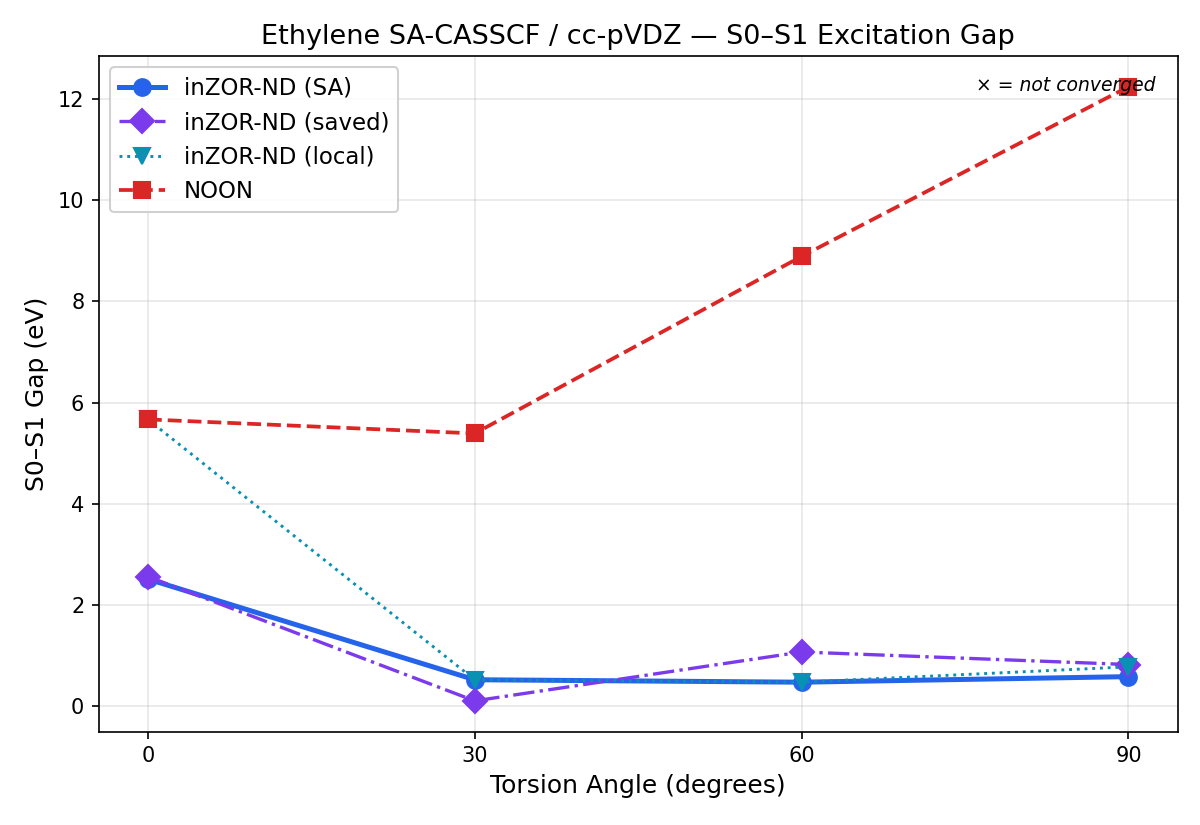
\includegraphics[width=0.92\linewidth]{ethylene_s0s1_gap.png}
  \caption{S$_0$--S$_1$ gap visual (ethylene quasi-degeneracy study, exported
  from the inZOR-ND validation workspace).}
  \label{fig:eth1}
\end{figure}

\begin{figure}[htbp]
  \centering
  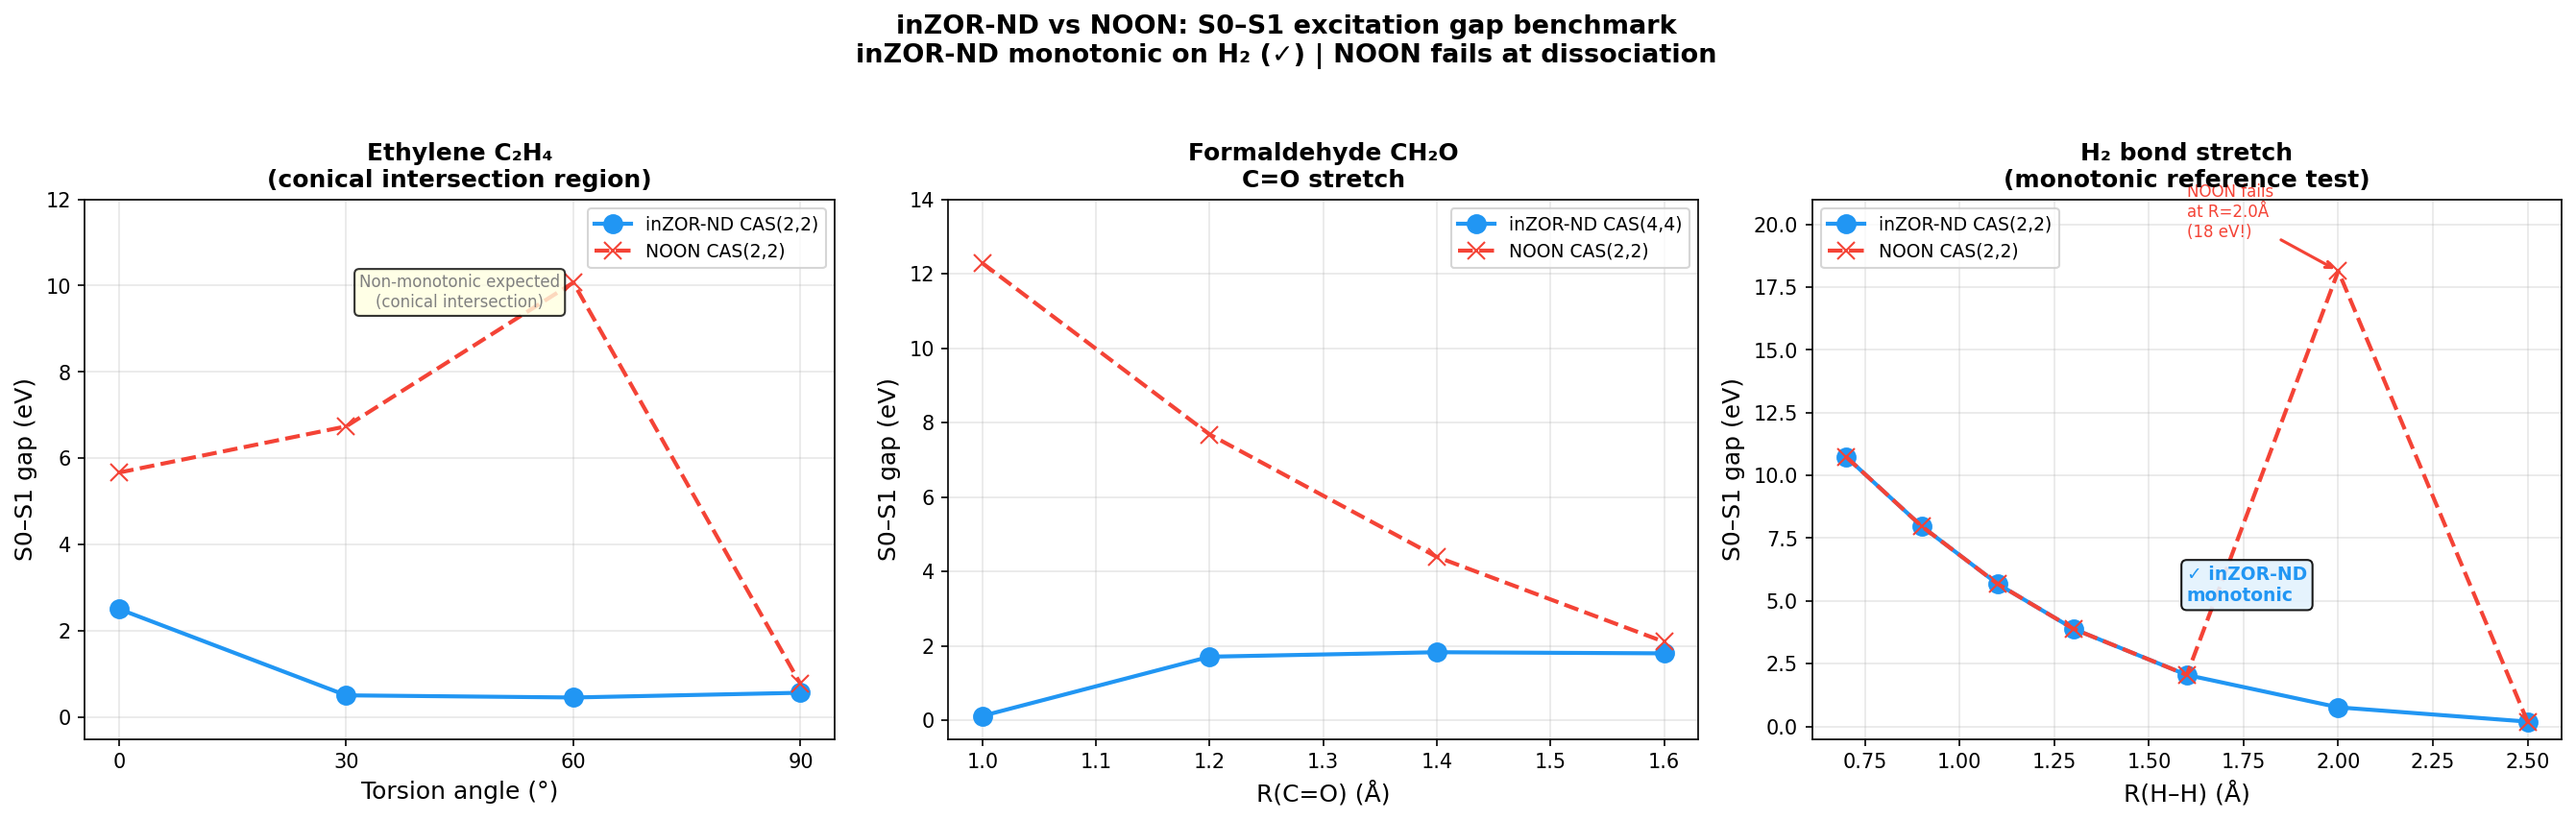
\includegraphics[width=0.92\linewidth]{vladimir_final_comparison.png}
  \caption{Validation-style comparison across batches or score variants
  (ethylene thread export).}
  \label{fig:eth2}
\end{figure}

\begin{figure}[htbp]
  \centering
  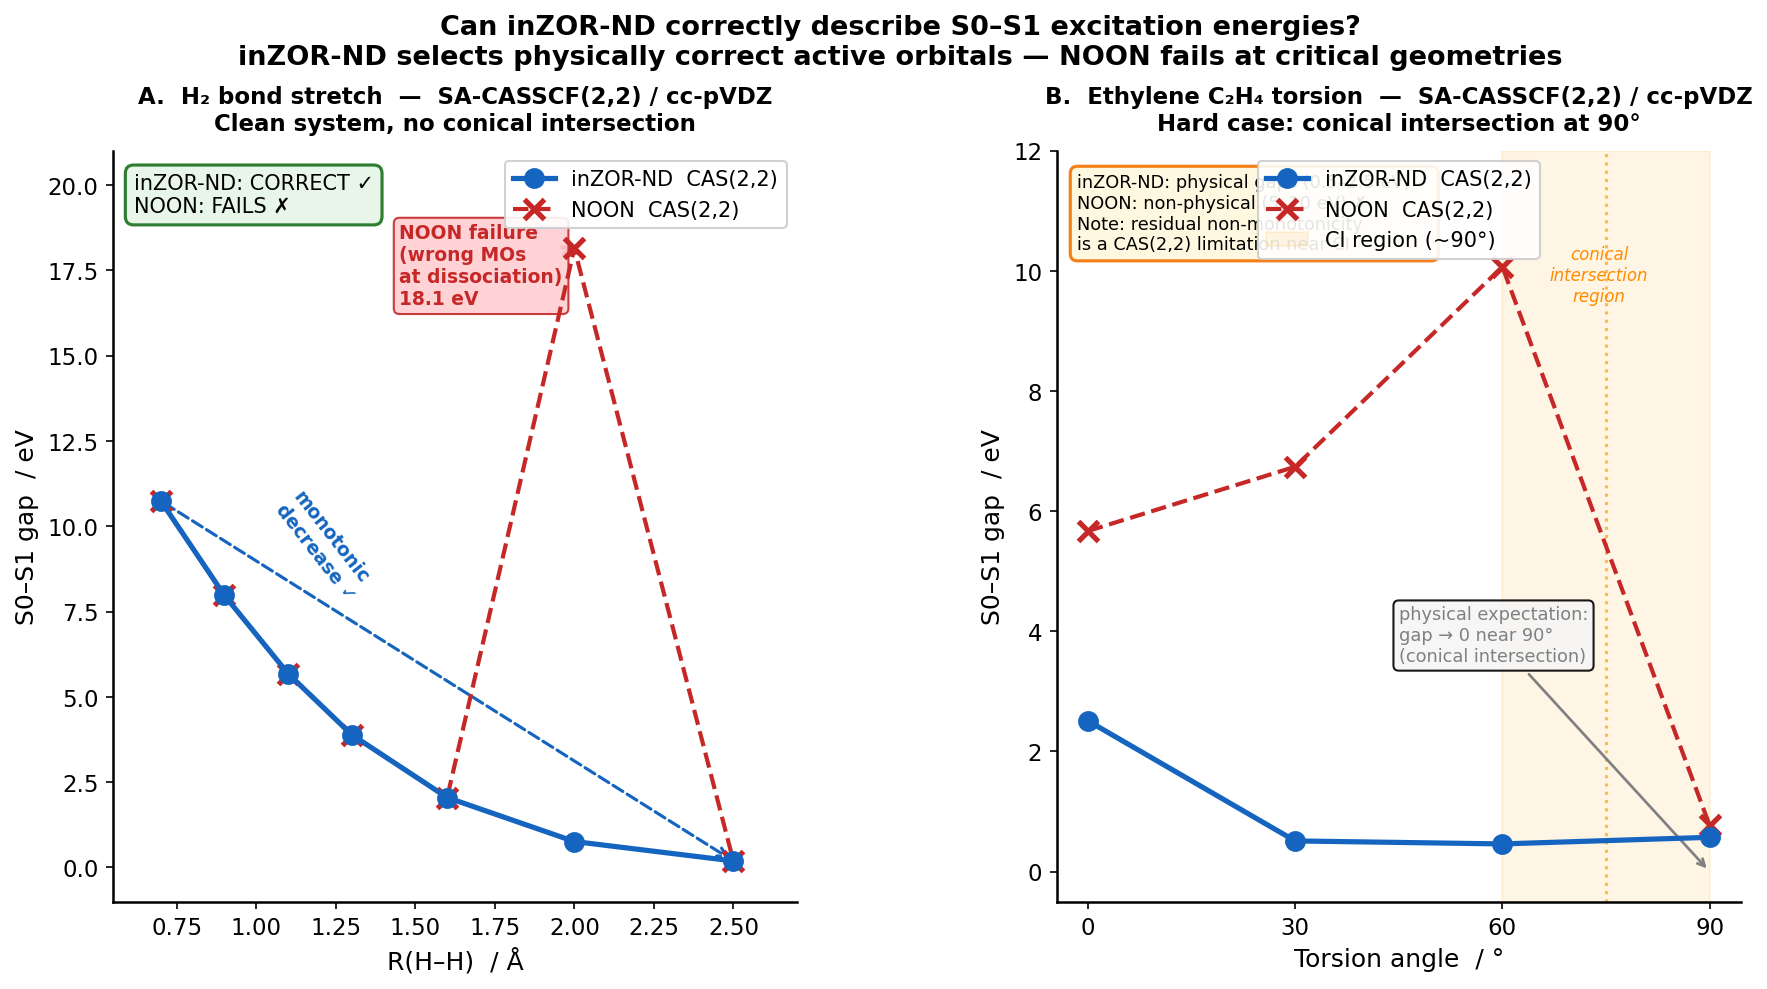
\includegraphics[width=0.92\linewidth]{vladimir_answer.png}
  \caption{Companion metrics / reference panel for the same validation workflow.}
  \label{fig:eth3}
\end{figure}

\section{Relation to discrete-search benchmarks}
The \textbf{eight-benchmark} interactive report treats ethylene SA-CASSCF within
a \textbf{discrete-search} protocol against NOON-MP2 / AVAS-style
baselines~\citep{inZORNDActiveSpace2026}. The present unified chapter adds (i) a
\textbf{minimal H$_2$ gap sanity check} for orbital heuristics and (ii) a
\textbf{continuous exploration} narrative for ethylene. Readers should cite the
comparative suite for large-molecule CAS discovery statistics, and this note for
gap-focused motivation, the H$_2$ table, and the exploration/validation figures.

\section{Reproducibility}
\textbf{H$_2$:} regenerate from the driver that produced
\texttt{h2\_stretch\_results.json}; pin PySCF and dependencies for bit-identical
replication if required.

\textbf{Ethylene:} scene assets, exports, and validation logs live under
\texttt{zor\_scenes/scene\_ethylene\_quasidegen/} in the source repository
referenced from the public HTML~\citep{inZORNDQCGaps2026}.

\textbf{3D regional batch:} named validation directories and JSON summaries are
listed on the 3D page~\citep{inZORNDEthylene3D2026}; reproducibility of
clustering is demonstrated for \textbf{byte-identical} \texttt{probes.jsonl}
reruns, not for independent stochastic trajectories.

\section{Conclusion}
Quasi-degenerate regimes demand scrutiny of \textbf{gap observables}, not only
total energies. A seven-point H$_2$ scan separates inZOR-ND and NOON-style
orbital choices on a transparent curve: one track stays monotone; the other
breaks down at an intermediate bond length. In parallel, ethylene provides a
richer geometry where inZOR-ND continuous exploration couples SA-CASSCF(2,2)
gaps to population dynamics, with extended regional analysis in a dedicated 3D
report. Keeping \textbf{discrete-search} and \textbf{continuous-exploration}
claims apart preserves scientific hygiene as both lines evolve.

\section*{Data and code availability}
Interactive report (HTML): \url{https://dumitrunovic-svg.github.io/inZOR-ND/tests/qc_gaps_h2_ethylene_unified/}.\\
Ethylene 3D technical page: \url{https://dumitrunovic-svg.github.io/inZOR-ND/tests/qc_gaps_h2_ethylene_unified/ethylene_3d_zor.html}.\\
Repository (tests and brochure source): \url{https://github.com/dumitrunovic-svg/inZOR-ND}.

\bibliographystyle{unsrtnat}
\bibliography{references}

\end{document}
